\documentclass[11pt,a4paper,twoside]{ipb}
    %\usepackage{showframe}
    \usepackage{eec}
\usepackage[portuguese]{babel}%pacote linguagem
\usepackage{lastpage}%pacote para indicar a ultima pagina do documento
\usepackage{csquotes}
\graphicspath{{./images/}}
\usepackage{listings} % incluir listagens
\usepackage{url} % typeset URL's
\usepackage[colorlinks=true,
            %urlcolor=azuel, %azul escuro
             urlcolor=blue, %blue
             linkcolor=black,
             citecolor=blue, %cor das citações
             bookmarks=true,
            pdfstartview=FitH]{hyperref}
\usepackage{cleveref} 
\bibliographystyle{plainnat}%estilo da bibliografica
\usepackage[backend=biber,
            style=numeric,
            sorting=ynt,
            %dashed=false,
            autolang=other,
            bibencoding=UTF8,]{biblatex} % config da bibliografia
\addbibresource{refs.bib} %input da bibliogradia
\usepackage{lipsum}
%\usepackage[pdftex]{hyperref}
\usepackage{tabulary} % pacote para tabelas
\usepackage{amsmath,amssymb,amsfonts,textcomp} % vários pacotes juntos, utilizados para usar funções e outros símbolos matemáticos
\usepackage{indentfirst} % indenta todo 1º parágrafo
\usepackage{float}% força as figuras a ficarem depois do texto.
\usepackage{placeins}% força as figuras a ficarem depois do texto.
\FloatBarrier
\usepackage{subfigure}% pacote para sfubfigures
\usepackage{multirow} % pacote para utilizar multirow nas tabelas
\usepackage{afterpage}
\usepackage{pdfpages} %pacote para incluir pdf no documento
\usepackage{mathtools} 
\usepackage{booktabs}
\usepackage{siunitx} % pacote para incluir as unidade do sistema internacional
%\usepackage{scrextend}
\listfiles
\usepackage{changepage}
\usepackage{titlesec} %pacote para \titleformat
\usepackage[font=footnotesize,labelfont=bf]{caption} %config de todos os \caption
\usepackage{tikz}
\usetikzlibrary{calc}
\usepackage{multicol}
\usepackage{tzplot}
\usepackage{pgfplots}
\pgfplotsset{compat=newest}
\usepgfplotslibrary{groupplots}
\usepgfplotslibrary{dateplot}
\usepackage{comment}
%\usepackage[Bjornstrup]{fncychap}
     \renewcommand*{\lstlistlistingname}{Lista de Algoritmos}
    %%%%%%%%%%%%%%%%%%%%%%%%% Dados %%%%%%%%%%%%%%%%%%%%%%%%%%%%%%%%%%%%%% 
    \title{T\'{i}tulo do Projeto}
    \author{Nome completo do Aluno}
    \supervisor{Professor Doutor Nome do Orientador}
    \cosupervisor{Engenheiro Nome do Co-Orientador} %nome do tutor da empresa
    \course{Engenharia Eletrot\'{e}cnica e de Computadores}
    \courseyear{\ano}
    %\courseyear{\today}
    %%%%%%%%%%%%%%%%%%%%%%%%%%%%%%%%%%%%%%%%%%%%%%%%%%%%%%%%%%%%%%%%%%%%%%%
    %%%%%%%%%%%%%%%%%%%%%%%%% Lista de Símbolos %%%%%%%%%%%%%%%%%%%%%%%%%%%   
    %\setlength{\glsdescwidth}{15cm}
    \setlength\glsdescwidth{0.75\hsize}
    \newglossary[slg]{symbolslist}{syi}{syg}{Nomenclatura} % create and add. symbolslist
    \glsaddkey{unit}{\glsentrytext{\glslabel}}{\glsentryunit}{\GLsentryunit}{\glsunit}{\Glsunit}{\GLSunit}
    %%%%%%%%%%%%%%%%%%%%%%%%%%%%%%%%%%%%%%%%%%%%%%%%%%%%%%%%%%%%%%%%%%%%%%%
    
    %%%%%%%%%%%%%%%%%%%%%%%%% Print: %%%%%%%%%%%%%%%%%%%%%%%%%%%%%%%%%%%%%%  
    \makeglossaries 
    \newglossaryentry{p}{name=\ensuremath{P},
        description={Potência Ativa},
        unit={\si{W}},
        type=symbolslist}
\newglossaryentry{i}{name=\ensuremath{I},
        description={Corrente},
        unit={\si{A}},
        type=symbolslist} 
\newglossaryentry{ii}{name=\ensuremath{I_N},
        description={Corrente Nominal},
        unit={\si{A}},
        type=symbolslist}
 \newglossaryentry{iii}{name=\ensuremath{I'},
        description={Corrente para o Rendimento Máximo},
        unit={\si{A}},
        type=symbolslist}
 \newglossaryentry{f}{name=\ensuremath{f},
        description={Frequência},
        unit={\si{Hz}},
        type=symbolslist}       
\newglossaryentry{s}{name=\ensuremath{S},
        description={Potência Aparente},
        unit={\si{VA}},
        type=symbolslist}        
\newglossaryentry{q}{name=\ensuremath{Q},
        description={Potência Reativa},
        unit={\si{var}},
        type=symbolslist}
\newglossaryentry{us}{name=\ensuremath{U_s},
        description={Tensão Simples},
        unit={\si{V}},
        type=symbolslist}
\newglossaryentry{uc}{name=\ensuremath{U_c},
        description={Tensão Composta},
        unit={\si{V}},
        type=symbolslist}  
\newglossaryentry{z}{name=\ensuremath{Z},
        description={Impedância},
        unit={$R+jX$~\si{\Omega}},
        type=symbolslist}
\newglossaryentry{n}{name=\ensuremath{\eta},
        description={Rendimento},
        unit={\%},
        type=symbolslist}        
 %-Lista de Símbolos
    \loadglsentries{listas/acronym} %-Lista de Acrónimos
    %%%%%%%%%%%%%%%%%%%%%%%%%%%%%%%%%%%%%%%%%%%%%%%%%%%%%%%%%%%%%%%%%%%%%%%
    
    %%%%%%%%%%%%%%%%%%%%%%%%% Lista de Símbolos %%%%%%%%%%%%%%%%%%%%%%%%%%% 
    \newglossarystyle{symbunitlong}{
    \setglossarystyle{long3col}
    
    \renewenvironment{theglossary}{% Muda o tipo da tabela
    \renewcommand{\arraystretch}{1.5}    
    \begin{longtable}{cp{0.5\glsdescwidth}>{\centering\arraybackslash}p{2cm}}}%
    {\end{longtable}}%
    \renewcommand*{\glossaryheader}{\toprule %Muda a 1ª linha da tabela
    \bfseries S\'{i}mbolo&\bfseries Descri\c{c}\~{a}o&\bfseries{\itshape SI}\\\midrule\endhead }
    \renewcommand*{\glossentry}[2]{%Muda os itens
    \glstarget{##1}{\glossentryname{##1}}
    & \glossentrydesc{##1}%Descricao
    & \glsunit{##1}  \tabularnewline}
    }
    %%%%%%%%%%%%%%%%%%%%%%%%%%%%%%%%%%%%%%%%%%%%%%%%%%%%%%%%%%%%%%%%%%%%%
    
    \begin{document}
        %%%%%%%%%%%%%%%%%%%%%%%% Define color %%%%%%%%%%%%%%%%%%%%%%%%%%%
        \definecolor{azuel}{rgb}{0.07, 0.04, 0.56}
        \definecolor{backcolour}{rgb}{0.95,0.95,0.92}
        \definecolor{codegreen}{rgb}{0,0.6,0}
        \definecolor{mygreen}{RGB}{28,172,0}
        \definecolor{mylilas}{RGB}{170,55,241}
        \definecolor{codegray}{rgb}{0.5,0.5,0.5}
        \definecolor{codepurple}{rgb}{0.58,0,0.82}
        %%%%%%%%%%%%%%%%%%%%%%%%%%%%%%%%%%%%%%%%%%%%%%%%%%%%%%%%%%%%%%%%%
        
        %%%%%%%%%%%%%%%%%%%%%%%%% Config List %%%%%%%%%%%%%%%%%%%%%%%%%%% 
        \lstdefinestyle{list1}{backgroundcolor=\color{backcolour},   
                            commentstyle=\color{codegreen},
                            %keywordstyle=\footnotesize\color{magenta},
                            keywordstyle=\footnotesize\color{blue},
                            numberstyle=\footnotesize\color{black},
                            stringstyle=\footnotesize\color{codepurple},
                            basicstyle=\footnotesize,
                            breakatwhitespace=false,
                            frame=single,
                            breaklines=true,                 
                            keepspaces=true,                 
                            numbers=left,       
                            numbersep=10pt,                  
                            showspaces=false,                
                            showstringspaces=false,
                            showtabs=false,                  
                            tabsize=2,}
                            
        \lstdefinestyle{list2}{language=Matlab,% lst
                                 %basicstyle=color{red},
                                 backgroundcolor=\color{white},
                                 breaklines=true,
                                 breakatwhitespace=false,
                                 keepspaces=true,
                                 morekeywords={matlab2tikz},
                                 showspaces=false, 
                                 showtabs=false,
                                 tabsize=2,
                                 %frame=single,
                                 keywordstyle={\footnotesize\color{blue}},
                                 morekeywords=[2]{1}, 
                                 keywordstyle=[2]{\footnotesize\color{black}},
                                 identifierstyle={\footnotesize\color{black}},%
                                 stringstyle={\footnotesize\color{mylilas}},
                                 commentstyle={\footnotesize\color{mygreen}},
                                 showstringspaces=false,
                                 numbers=left,%
                                 numberstyle={\footnotesize\color{black}},
                                 numbersep=10pt, 
                                 emph=[1]{for,end,break},emphstyle=[1]\footnotesize\color{blue}, 
                                 }
        %%%%%%%%%%%%%%%%%%%%%%%%%%%%%%%%%%%%%%%%%%%%%%%%%%%%%%%%%%%%%%%%%%%%%%
        \def\ano{\expandafter\YEAR\the\year}\def\YEAR#1#2#3#4{#1#2#3#4} %Coloca ano automatico
        
        %%%%%%%%%%%%%%%%%%%%%%%%% Config Equations %%%%%%%%%%%%%%%%%%%%%%%%%%% 
        \makeatletter % make "@" a letter-type symbol
            \providecommand\add@text{}
            \newcommand\addunit[1]{%
            \gdef\add@text{(\si{#1})\gdef\add@text{}}}
            \def\tagform@#1{\maketag@@@{(Eq.~#1\unskip\@@italiccorr)}}
            \renewcommand*{\@biblabel}[1]{\hfill#1.}
        \makeatother
        \newtagform{Eq}[\upshape]{\footnotesize\textbf{Eq.~}}{}\usetagform{Eq}
        \renewcommand\theequation{{\bfseries\footnotesize\thechapter.\bfseries\arabic{equation}}}
        %%%%%%%%%%%%%%%%%%%%%%%%%%%%%%%%%%%%%%%%%%%%%%%%%%%%%%%%%%%%%%%%%%%%%%%
        
        %%%%%%%%%%%%%%%%%%%%%%%%% Config titles %%%%%%%%%%%%%%%%%%%%%%%%%%%%%%%
         %\titleformat{\chapter}[hang]{\normalfont\huge\bfseries}{\thechapter.}{0.5cm}{\filright} %\titlespacing{\chapter}{0em}{0.5cm}{1.5cm}   
        \titleformat{\chapter}[display]{\normalfont\huge\bfseries}{\chaptertitlename~\thechapter.}{1ex}{\filright}
        \titleformat{\section}[hang]{\normalfont\Large\bfseries}{\thesection.}{1ex}{}
        \titleformat{\subsection}[hang]{\normalfont\large\bfseries}{\thesubsection.}{1ex}{}
        \titleformat{\subsubsection}[hang]{\normalfont\bfseries}{}{1ex}{}
        %%%%%%%%%%%%%%%%%%%%%%%%%%%%%%%%%%%%%%%%%%%%%%%%%%%%%%%%%%%%%%%%%%%%%%%
        
        %%%%%%%%%%%%%%%%%%%%%% Config Cabeçalho %%%%%%%%%%%%%%%%%%%%%%%%%%%%%%%
        \renewcommand{\sectionmark}[1]{\markright{\thesection.~#1}}
        \renewcommand{\chaptermark}[1]{\markboth{\thechapter.~#1}{}}
        %%%%%%%%%%%%%%%%%%%%%%%%%%%%%%%%%%%%%%%%%%%%%%%%%%%%%%%%%%%%%%%%%%%%%%%
        
        %%%%%%%%%%%%%%%%%%%% Config Nota Rodapé  %%%%%%%%%%%%%%%%%%%%%%%%%%%%%%
        \newcounter{tempfootnote}
        \setcounter{footnote}{\value{tempfootnote}}
        \renewcommand{\thefootnote}{\bfseries\arabic{footnote}}
        %%%%%%%%%%%%%%%%%%%%%%%%%%%%%%%%%%%%%%%%%%%%%%%%%%%%%%%%%%%%%%%%%%%%%%%
        
        %%%%%%%%%%%%%%%%%%%%%%%%% Config \Ref %%%%%%%%%%%%%%%%%%%%%%%%%%%%%%%%%
        \let\origref\ref
        \def\ref#1{\textbf{\origref{#1}}}
        %%%%%%%%%%%%%%%%%%%%%%%%%%%%%%%%%%%%%%%%%%%%%%%%%%%%%%%%%%%%%%%%%%%%%%%

        \renewcommand{\lstlistingname}{Algoritmo}
        
        \beforepreface
        \pagenumbering{roman}
        \chapter*{Dedicat\'{o}ria}
            \markboth{Dedicat\'{o}ria}{}
            (Facultativo) Dedico este trabalho a ...
        \cleardoublepage
        \chapter*{Agradecimentos}
            \markboth{Agradecimentos}{}
            (Facultativo) Agradeço este trabalho a ...
        \cleardoublepage    
        \prefacesection*{Resumo}
            \markboth{Resumo}{}
            O resumo (no máximo com 250 palavras), permite a avaliação do interesse de um documento e facilita a sua identificação na pesquisa bibliográfica em bases de dados onde o documento se encontre referenciado. 

É recomendável que o resumo aborde, de forma sumária:
\begin{itemize}
	\item Objetivos principais e tema ou motivações para o trabalho; 
	\item Metodologia usada (quando necessário para a compreensão do relatório); 
	\item Resultados, analisados de um ponto de vista global; 
	\item Conclusões e consequências dos resultados, e ligação aos objetivos do trabalho.
\end{itemize}

Como este modelo de relatório se dirige a trabalhos cujo foco incide, maioritariamente, no desenvolvimento de software, algumas destas componentes podem ser menos enfatizadas, e acrescentada informação sobre análise, projeto e implementação do trabalho.

O resumo não deve conter referências bibliográficas.

\mbox{}\linebreak
\noindent {\bf Palavras-chave:} termos (no máximo 4), que descrevem o trabalho.

        \cleardoublepage
        \prefacesection*{Abstract}
            \markboth{Abstract}{}
            Direct translation (maximum of 250 words) to English of the section ``Resumo''.

\mbox{}\linebreak
\noindent {\bf Keywords:} direct translation of ``Palavras-chave''

        \cleardoublepage
        
        \afterpreface
        
       \glsaddall %para colocar todos os gls
        \cleardoublepage
        \printglossary[type=\acronymtype,title={Acr\'{o}nimos e Siglas},nonumberlist] % print e edita o titulo
        \cleardoublepage
        \printglossary[type=symbolslist,title={Nomenclatura},style=symbunitlong] % print e edita o titulo
	    \cleardoublepage
     
        \bodystart
                           
        \chapter{Introdução}\label{cap1}

Este documento pretende guiar o Estudante na elaboração do relatório de Projeto/Estágio, do 3º ano da \gls{ESTIG} do \gls{IPB} a frequentar o curso de \gls{EEC}.\par
O autor deverá ter em consideração as seguintes regras gerais na elaboração do documento:
\begin{itemize}
	\item O documento deve ser redigido em português ou inglês com um estilo adequado e correto do ponto de vista gramatical (quer do ponto de vista sintático quer semântico);
	\item Ter especial cuidado com o uso de adjetivos (facilmente conduzem ao exagero), advérbios (nada, ou quase nada, acrescentam) e sinais de pontuação (em especial o uso correto das vírgulas);
	\item O estilo adotado para a redação deve ser coerente com as exigências de um trabalho científico encontrado em publicações impressas;
	\item De uma forma genérica deve usar a 3ª pessoa do singular (eventualmente do plural), exceção feita aos locais onde tal \'e claramente desajustado, por exemplo, na secção dos agradecimentos;
	\item Usar o estilo \textit{it\'{a}lico} sempre que s\~ao utilizados termos em l{\'i}nguas diferentes da l{\'i}ngua adotada no relat{\'o}rio, para escrever símbolos matemáticos, por exemplo $\omega$, ou \textit{$\omega$};
	\item O uso de acr\'onimos implica que na 1ª vez que são utilizados se apresentem por extenso, colocando entre parênteses a respetiva sigla que se passará a usar. Todos os acrónimos devem ser apresentados por ordem alfabética na secção ``Lista de Acrónimos'';
    	\item O uso correto de unidades, seus múltiplos e submúltiplos \footnote{As unidades utilizadas ao longo do relatório deverá ser introduzida em \textbf{Nomenclatura}.};
	\item As imagens e tabelas devem, por princípio, aparecer no topo ou no fundo da página. A legendas  das figuras surgem imediatamente após as figuras e no caso das tabelas as legendas antecedem as mesmas;
	\item Todas as figuras, tabelas e restantes listagens devem ser mencionadas no texto por forma a que fiquem enquadradas nas ideias transmitidas pelo autor. Esta referência, regra geral, deverá ser feita antes da ocorrência da figura, tabela ou listagem;
	\item Indicar ao longo do texto as referências documentais usadas, em especial nas citações (puras ou literais), assinaladas com a utilização de aspas, como também no caso de reutilização de gráficos, figuras, tabelas, fórmulas, etc., de outras fontes;
\end{itemize}

De uma forma já mais específica, neste primeiro capítulo obrigatório (``Introdução'') o autor deve \footnote{Recomenda-se para cada item a utilização de uma secção}:
\begin{itemize}
	\item Contextualizar a proposta de trabalho no âmbito da empresa, de um outro trabalho já realizado, do ponto de vista científico e/ou tecnológico, etc.;
	\item Apresentar de forma clara os objetivos que se propõe atingir;
	\item Descrever de forma sucinta, mas objetiva, a solução preconizada ou a hipótese colocada;
	\item Apresentar de forma resumida, mas clara, os desenvolvimentos efetuados;
	\item Identificar como foi validada e avaliada a solução encontrada;
	\item Descrever a organização do documento.
\end{itemize}

        \cleardoublepage
        \chapter{Contexto e Tecnologias/Ferramentas}\label{cap2}

\begin{adjustwidth}{2.5cm}{0.3cm}
Nunca colocar uma $section$ depois de um $chapter$ por isso, aqui deve-se fazer um breve resumo do que se vai falar ao longo do capítulo (2 - 3 linhas), por exemplo....
Neste capítulo será abordado formas de incluir figuras, tabelas e equações.
\end{adjustwidth}

\section{Figuras}
Nesta secção será abordado como poderá-se colocar um figura num documento $Latex$.\par
De acordo com \cite{overleaf}, em $Latex$ Básico que para incluir figuras é necessário o pacote $graphicx$, que já está introduzido no ficheiro `` package.text''. Posto isto, ao longo do capítulo é importante referir o significado da figura, como por exemplo ``Na Figura \ref{fig:leon} será ilustrado um exemplo de uma figura''. Em segundo a legenda de uma figura fica  \underline{sempre} depois da figura.
\begin{figure}[htpb]
    \centering
    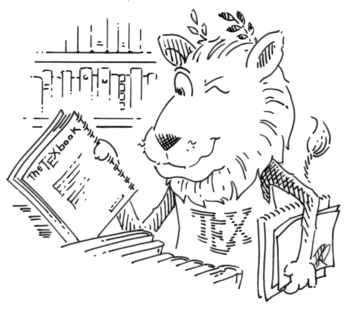
\includegraphics[scale=0.4]{imagens/lion_large.png}
    \caption{Exemplo de uma figura.}
    \label{fig:leon}
\end{figure}\par 
Por vezes é necessário colocar 2 figuras simumltaneamente como será ilustrada na figura \ref{fig:leon1}
\begin{figure}[H]
    \centering
    \subfigure[Figura 1]{\label{plot1}
    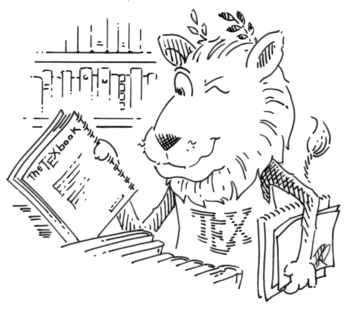
\includegraphics[scale=0.4]{imagens/lion_large.png}
    }\hspace{.5cm}
    \subfigure[Figura 2]{\label{plot2}
    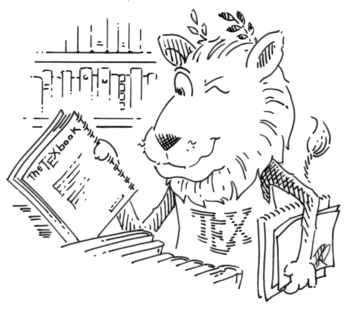
\includegraphics[scale=0.4]{imagens/lion_large.png}
    }
    \caption{Figuras apresentadas com o pacote $subfigure$.}
    \label{fig:leon1}
\end{figure}\par
Na Figura \ref{fig:leon1} cada sub-figura têm uma sub-legenda, na Figura \ref{fig:_lado_a_lado} será ilustrado duas Figura com apenas uma legenda.
\begin{figure}[H]
    \centering
    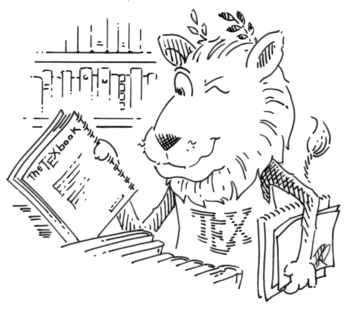
\includegraphics[scale=0.4]{imagens/lion_large.png} \ \ \ \ \ \ \
    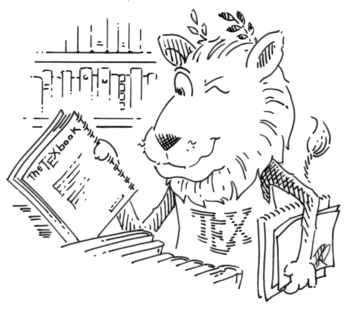
\includegraphics[scale=0.4]{imagens/lion_large.png}
    \caption{Exemplo de duas figuras, uma ao lado da outra.}
    \label{fig:_lado_a_lado}
\end{figure}

\section{Tabelas}
Nesta secção será abordado como poderá-se colocar um tabela num documento $Latex$.\par
Segundo \cite{overleaftables}, uma tabela é definida entre os comandos \verb|\begin{tabular}| e \verb|\end{tabular}|, já seguir será ilustrado um exemplo.\par
\begin{table}[H]
    \renewcommand{\arraystretch}{1.5}
    \centering
    \caption{Tabela centralizada.}
    \label{tab1}
    \begin{tabular}{ccc}
        \hline
        Coluna  & Coluna  & Coluna \\
        \hline
        a & b & c \\
        d & e & f \\
        \hline
    \end{tabular}
\end{table}\par
Após \verb|\begin{tabular}| é colocado, entre \verb|{}|, ccc, o que indica que a tabela terá 3 colunas, todas centralizadas. O número de letras indica o número de colunas e a letra o seu alinhamento: 
\begin{itemize}
    \item c para colunas com texto alinhado centralizado;
    \item l para colunas com texto alinhado à esquerda;
    \item r para colunas com texto alinhado à direita.
\end{itemize}\par
Para indicar uma separação de coluna use-se \verb|&|. Para indicar o número linhas usa-se duas
barras juntas, \verb|\\|, o que significa quebra de linha. O comando \verb|\hline| é responsável por colocar uma linha horizontal na tabela e o comando \verb|\cline{-}| faz uma linha horizontal somente entre as colunas indicadas. Para inserir linhas verticais usa-se \verb||| entre as letras que indicam o alinhamento da coluna.
\begin{table}[H]
    \renewcommand{\arraystretch}{1.5}
    \centering
    \caption{Tabela com alinhamento à esquerda.}
    \label{tab2}
    \begin{tabular}{|l|cc|}
    \hline
    Coluna & Coluna  & Coluna \\
    \hline \hline
    A & B & C \\
    \cline{2-3}
    D & E & F \\
    \hline
    \end{tabular}
\end{table}\par 
Se uma coluna receber um texto longo e seja necessário que haja uma quebra de linha dentro da célula, em vez de usar as letras c, l ou r usa-se \verb|p{}|, onde dentro \verb|{}| incluiu-se o tamanho da linha.
\begin{table}[H]
    \renewcommand{\arraystretch}{1.5}
    \centering
    \caption{Tabela usando $p\{\}$.}
    \label{tab3}
    \begin{tabular}{ccp{5cm}}
    \hline
    C & C & Coluna de Texto \\
    \hline
    A & B & Aqui será digitado um texto grande,
    mas a largura da célula é fixa em 5 \si{\cm}.\\
\hline
\end{tabular}
\end{table}\par
É possível tornar as tabelas mais bonitas, para isso é necessário  usar \verb|\usepackage{booktabs}|, ou seja este pacote retira o \verb|\hline| e coloca: 
\begin{itemize}
    \item \verb|\toprule|, para a linha superior da tabela;
    \item \verb|\midrule|, para as linhas no meio da tabela;
    \item \verb|\bottomrule|, para a linha abaixo da tabela.
\end{itemize}
\begin{table}[H]
    \renewcommand{\arraystretch}{1.15}
    \centering
    \caption{Tabela usando o pacote $booktabs$.}
    \label{tabela3}
    \begin{tabular}{llr}
        \toprule
        \multicolumn{2}{c}{Item} \\
        \cmidrule(r){1-2}
        Animal & Description & Price (\$)\\ \midrule
        Gnat & per gram & 13.65 \\
        & each & 0.01 \\
        Gnu & stuffed & 92.50 \\
        Emu & stuffed & 33.33 \\
        Armadillo & frozen & 8.99 \\
        \bottomrule
    \end{tabular}
\end{table}


\section{Equações}
Em qualquer fórmula matemática existem constantes e variáveis, o $Latex$ adota como convenção de
trabalho, modificar a fonte e a apresentação dos elementos em função do seu tipo, constante ou variável, como por exemplo  $p''=max\{f(y),g(x)\}$ \footnote{Sempre que iniciar uma equação é obrigatório ter legenda ``Eq.2.1''.}.
\begin{equation}
    f_X(x) = \frac{1}{\sqrt{2 \pi \sigma^2}}e^{-\frac{(x-\mu)^2}{2\sigma^2}}
\end{equation}
\begin{equation*}
    f_X(x) = \frac{1}{\sqrt{2 \pi \sigma^2}}e^{-\frac{(x-\mu)^2}{2\sigma^2}}
\end{equation*}
\begin{center}
    $f_X(x) = \frac{1}{\sqrt{2 \pi \sigma^2}}e^{-\frac{(x-\mu)^2}{2\sigma^2}}$
\end{center}\par
Para mais informações \cite{overleafsimbolos,simbolos}.

        \cleardoublepage
        \chapter{Abordagem/Análise/Modelação}\label{cap3}
\begin{adjustwidth}{2.5cm}{0.3cm}
Neste capítulo espera-se uma descrição detalhada do problema e da proposta de solução. 
\end{adjustwidth}

        \cleardoublepage
        \input{capitulos/cap4}
        \cleardoublepage
        \chapter{Conclusão}\label{cap5}

As conclusões devem sintetizar e proporcionar uma perspetiva unificadora ao trabalho efetuado. Poderá ser feita uma breve referência a trabalhos de outros com semelhanças ao efetuado e ao conhecimento que resultou do trabalho efetuado, bem como sugestões de trabalho futuro. A coerência do documento implica que as conclusões devem ser coerentes com as ideias expostas na introdução.
        \cleardoublepage
        \printbibliography 
        \cleardoublepage
    
        \appendix % print anexos

        \pretocmd{\chapter}{\pagenumbering{arabic}
	                          \renewcommand*{\thepage}{\thechapter.\arabic{page}}
                           }{}{} 
        \chapter{Projeto}\label{anexo1}
\lstset{style=list1}
\lstinputlisting[caption=Simples código em $C++$, label={lstc}, language=C++]{codigos/codigo_c.cpp}

\lstset{style=list2}
\lstinputlisting[caption=Simples código em $Matlab$, label={lstmatlab}, language=Matlab]{codigos/exer2.m}





        \cleardoublepage
        \input{capitulos/anexo2.tex} 
        \cleardoublepage
        
\end{document}
